\section{El grupo fundamental}
\begin{ejercicio}
    Prueba que en un espacio topológico simplemente conexo $X$, dos arcos cualesquiera $\alpha,\beta\in \Omega(X,x,y)$ son homotópicos por arcos.\\

    \noindent
    Sean $\alpha,\beta\in \Omega(X,x,y)$, tenemos que $\alpha\ast\tilde{\beta}$ es un lazo basado en $x$, y por ser $X$ simplemente conexo tenemos que $\left[\alpha\ast\tilde{\beta}\right] = [\varepsilon_x]$, de donde:
    \begin{equation*}
        [\alpha]\ast\left[\tilde{\beta}\right] = \left[\alpha\ast\tilde{\beta}\right] = [\varepsilon_x] \Longrightarrow [\alpha] = [\beta]
    \end{equation*}
\end{ejercicio}

\begin{ejercicio}
    Sean $X$ un subconjunto de $\mathbb{R}^n$ y $f:X\to Y$ una aplicación. Demuestra que si $f$ se puede extender a una aplicación continua $F:\mathbb{R}^n\to Y$, entonces $f_\ast$ es el homomorfismo trivial, es decir, el homomorfismo que lleva todo elemento en el neutro.\\

    \noindent
    Como $F$ es una extensión de $f$, tenemos que $f\circ i = F$, es decir:
    \begin{figure}[H]
        \centering
        \shorthandoff{""}
        \begin{tikzcd}
            {X} \arrow[r, "i", hook] \arrow[rr, "f", bend right] & {\mathbb{R}^n} \arrow[r, "F"] & {Y}
        \end{tikzcd}
        \shorthandon{""}
    \end{figure}
    \noindent
    Y como cada una de ellas es continua ($f$ es continua por ser $f=F\big|_X$), podemos inducir el diagrama a grupos fundamentales, obteniendo para cada $x_0\in X$:
    \begin{figure}[H]
        \centering
        \shorthandoff{""}
        \begin{tikzcd}
            {\pi_1(X,x_0)} \arrow[r, "i_\ast", hook] \arrow[rr, "f_\ast", bend right=49] & {\pi_1(\mathbb{R}^n,x_0)} \arrow[r, "F_\ast"] & {\pi_1(Y,f(x_0))}
        \end{tikzcd}
        \shorthandon{""}
    \end{figure}
    de donde:
    \begin{equation*}
        f_\ast([\alpha]_X) = F_\ast(i_\ast([\alpha]_{X})) = F_\ast({[\alpha]}_{\bb{R}^n}) \AstIg F_\ast([\varepsilon_{x_0}]_{\mathbb{R}^n}) = [\varepsilon_{f(x_0)}]_Y \qquad \forall [\alpha]_X \in \pi_1(X,x_0)
    \end{equation*}
    donde en $(\ast)$ hemos usado que $\mathbb{R}^n$ es simplemente conexo.
\end{ejercicio}

\begin{ejercicio}
    Se dice que un grupo $G$ con operación $\cdot $ es un grupo topológico si $G$ tiene una topología de forma que las aplicaciones producto e inversión
    \Func{}{G\times G}{G}{(x,y)}{x\cdot y} \Func{}{G}{G}{x}{x^{-1}}
    son continuas. Sea e el elemento neutro en $G$:
    \begin{enumerate}[label=\alph*)]
        \item Dados $\alpha,\beta\in \Omega(G,e)$, se define $\alpha\cdot \beta:[0,1]\to G$ como $(\alpha\cdot \beta)(t) = \alpha(t)\cdot \beta(t)$. Demuestra que $\alpha\cdot \beta\in \Omega(G,e)$.

            Hemos de probar que $\alpha\cdot \beta$ es un lazo basado en $e$. Para ello:
            \begin{itemize}
                \item $\alpha\cdot \beta$ es continua, puesto que si consideramos:
                    \Func{\Phi}{G\times G}{G}{(x,y)}{x\cdot y}            
                    \Func{\Psi}{[0,1]}{G\times G}{t}{(\alpha(t), \beta(t))}
                    Tenemos que $\alpha\cdot \beta = \Phi \circ \Psi$:
                    \begin{equation*}
                        (\alpha\cdot \beta)(t) = \alpha(t)\cdot \beta(t) = \Phi(\alpha(t),\beta(t)) = \Phi(\Psi(t)) \qquad \forall t\in [0,1]
                    \end{equation*}
                    con $\Phi$ continua por hipótesis y $\Psi$ continua por ser $\Psi=(\alpha,\beta)$, con sus dos componentes funciones continuas, por ser arcos.
                \item Observemos que:
                    \begin{align*}
                        (\alpha\cdot \beta)(0) &= \alpha(0) \cdot \beta(0) = e\cdot e = e \\
                        (\alpha\cdot \beta)(1) &= \alpha(1) \cdot \beta(1) = e\cdot e = e \\
                    \end{align*}
            \end{itemize}
            Con lo que $\alpha\cdot \beta\in \Omega(G,e)$.
        \item Comprueba que $(\alpha\ast \varepsilon_e)\cdot (\varepsilon_e\ast \beta)=\alpha\ast \beta$ para cualesquiera $\alpha,\beta\in \Omega(G,e)$.

            Sean $\alpha,\beta\in \Omega(G,e)$, tenemos que:
            \begin{align*}
                ((\alpha\ast \varepsilon_e)&\cdot (\varepsilon_e\ast \beta))(t) = (\alpha\ast \varepsilon_e)(t)\cdot (\varepsilon_e\ast \beta)(t)  \\ &= \left\{\begin{array}{ll}
                    \alpha(2t)\cdot \varepsilon_e(2t) & \text{si\ } 0\leq t \leq \nicefrac{1}{2} \\
                    \varepsilon_e(2t-1)\cdot \beta(2t-1) & \text{si\ } \nicefrac{1}{2}\leq t \leq 1
                \end{array}\right.  \\
               &= \left\{\begin{array}{ll}
                   \alpha(2t)\cdot e & \text{si\ } 0\leq t \leq \nicefrac{1}{2} \\
                   e\cdot \beta(2t-1) & \text{si\ } \nicefrac{1}{2}\leq t\leq 1
           \end{array}\right\} = \left\{\begin{array}{ll}
               \alpha(2t) & \text{si\ } 0\leq t \leq \nicefrac{1}{2} \\
               \beta(2t-1) & \text{si\ } \nicefrac{1}{2}\leq t \leq 1
           \end{array}\right.\\ &= (\alpha\ast \beta)(t) \qquad \forall t\in [0,1]
            \end{align*}

        \item Sean $[\alpha],[\beta]\in \pi_1(G,e)$. Prueba que la operación $[\alpha]\cdot [\beta]=[\alpha\cdot \beta]$ está bien definida.

            Sean $\alpha,\alpha',\gamma,\gamma'\in \Omega(G,e)$ de forma que:
            \begin{equation}\label{eq:igualdades_ej3rel2}
                [\alpha] = [\alpha'], \qquad [\gamma] = [\gamma']
            \end{equation}
            hemos de probar que $[\alpha\cdot \gamma] = [\alpha'\cdot \gamma']$. De las igualdades~(\ref{eq:igualdades_ej3rel2}) sabemos que existen $H_1,H_2:[0,1]\times [0,1]\to G$ aplicaciones continuas con:
            \begin{gather*}
                H_1(s,0) = \alpha(s),\qquad  H_1(s,1) = \alpha'(s),\qquad  H_1(0,t) = e = H_1(1,t) \\
                H_2(s,0) = \gamma(s),\qquad  H_2(s,1) = \gamma'(s),\qquad  H_2(0,t) = e = H_2(1,t) 
            \end{gather*}
            Si definimos $H:[0,1]\times[0,1]\to G$ dada por:
            \begin{equation*}
                H(s,t) = H_1(s,t)\cdot H_2(s,t) \qquad \forall (s,t)\in [0,1]\times[0,1]
            \end{equation*}
            tenemos que $H$ es continua, ya que podemos verla como $H = \Phi\circ (H_1,H_2)$, al igual que inicmos en el apartado a), así como que:
            \begin{gather*}
                H(s,0) = H_1(s,0)\cdot H_2(s,0) = \alpha(s)\cdot \gamma(s) = (\alpha\cdot \gamma)(s) \\
                H(s,1) = H_1(s,1)\cdot H_2(s,1) = \alpha'(s)\cdot \gamma'(s) = (\alpha'\cdot \gamma')(s) \\
                H(0,t) = H_1(0,t)\cdot H_2(0,t) = e\cdot e = e = e\cdot e = H_1(1,t)\cdot H_2(1,t) = H(1,t)
            \end{gather*}
            Con lo que $H$ es una homotopía, lo que nos dice que $[\alpha\cdot \gamma] = [\alpha'\cdot \gamma']$, luego la operación está bien definida.
        \item Muestra que $[\alpha]\cdot [\beta]=[\alpha]\ast[\beta]$, para cada $[\alpha],[\beta]\in \pi_1(G,e)$.
            \begin{equation*}
                [\alpha]\cdot [\beta] = [\alpha\ast \varepsilon_e] \cdot [\varepsilon_e\ast \beta] = [(\alpha\ast\varepsilon_e)\cdot (\varepsilon_e\ast\beta)] \stackrel{b)}{=} [\alpha\ast\beta] = [\alpha]\ast [\beta]
            \end{equation*}
        \item Demuestra que $\pi_1(G,e)$ es abeliano.

            Sean $[\alpha],[\beta]\in \pi_1(G,e)$, tenemos que:
            \begin{align*}
                [\alpha]\ast[\beta] &= [\alpha\ast \beta] = [(\alpha\ast \varepsilon_e)\cdot (\varepsilon_e\ast \beta)] = [\alpha\ast \varepsilon_e] \cdot [\varepsilon_e\ast \beta]=  [\varepsilon_e\ast \alpha] \cdot [\beta\ast\varepsilon_e]  \\
                                    &= \left[ \left\{\begin{array}{ll}
                                         e\cdot \beta(2t)& \text{si\ } 0\leq t \leq \nicefrac{1}{2} \\
                                         \alpha(2t-1)\cdot e& \text{si\ } \nicefrac{1}{2}\leq t \leq 1
                             \end{array}\right.  \right] = [\beta\ast \alpha] = [\beta]\ast [\alpha]
            \end{align*}
    \end{enumerate}
\end{ejercicio}

\begin{ejercicio}
    Sean $X$ un espacio topológico y $f,g:X\to \bb{S}^n$ aplicaciones continuas con $g(x)\neq -f(x)$ para cada $x\in X$. Prueba que $f$ y $g$ son homotópicas. Deduce que si $f:\bb{S}^n\to \bb{S}^n$ es continua y carece de puntos fijos, entonces $f$ es homotópica a $-Id_{\bb{S}^n}$.\\

    \noindent
    Definimos $H:X\times [0,1]\to Y$ dada por:
    \begin{equation*}
        H(x,t) = \dfrac{(1-t)f(x) + tg(x)}{\|(1-t)f(x) + tg(x)\|_2} \qquad \forall (x,t)\in X\times [0,1]
    \end{equation*}
    \begin{itemize}
        \item $H$ está bien definida (es decir, el denominador no se anula), ya que si tenemos $x\in X$ y $t\in [0,1]$ de forma que $(1-t)f(x)+tg(x) = 0 $, entonces:
            \begin{equation*}
                (1-t)f(x) = -tg(x)
            \end{equation*}
            de donde:
            \begin{equation*}
                1-t = (1-t)\|f(x)\|_2 = \|(1-t)f(x)\|_2 = \|-tg(x)\|_2 = t\|g(x)\|_2 = t
            \end{equation*}
            por lo que ha de ser $t = \nicefrac{1}{2}$. Sin embargo, la condición $g(x)\neq -f(x)$ implica que $f(x) \neq -\nicefrac{1}{2}g(x)$, por lo que es imposible que el denominador se anule.
        \item $H$ es continua.
        \item Observamos que:
            \begin{equation*}
                H(x,0) = \dfrac{f(x)}{\|f(x)\|_2} = f(x) \qquad 
                H(x,1) = \dfrac{g(x)}{\|g(x)\|_2} = g(x) 
            \end{equation*}
    \end{itemize}
    con lo que $H$ es una homotopía entre $f$ y $g$.\\

    \noindent
    Sea ahora $f:\bb{S}^n\to \bb{S}^n$ una aplicación sin puntos fijos, entonces:
    \begin{equation*}
        f(x) \neq x = -(-x) = -(-Id_{\bb{S}^n})(x) \qquad \forall x\in \bb{S}^n
    \end{equation*}
    y si aplicamos la parte del ejercicio que acabamos de probar, obtenemos que $f$ es homotópica a $-Id_{\bb{S}^n}$.
\end{ejercicio}

\begin{ejercicio}\label{ej:1_top_triv}
    Sea $p:R\to B$ una aplicación recubridora y $b\in B$. Demuestra que el subespacio topológico $p^{-1}(\{b\})\subset R$ tiene la topología discreta.\\

    \noindent
    Sea $X = p^{-1}(\{b\})$, como $p$ es una aplicación recubridora, podemos tomar un abierto $O_b$ que contiene a $b$ y está regularmente recubierto, con lo que existen $\{A_i\}_{i \in I}$ conjuntos abiertos de $R$ de forma que:
    \begin{equation*}
        p^{-1}(O_b) = \biguplus_{i \in I}A_i
    \end{equation*}
    Sea $r\in X\subseteq p^{-1}(O_b)$, tenemos entonces que existe un índice $j\in I$ de forma que $r\in A_j$. Veamos que $A_j$ no puede contener dos elementos distintos de $X$, pues si $r,r'\in A_j\cap X$, tenemos que:
    \begin{equation*}
        p\big|_{A_j}(r) = b = p\big|_{A_j}(r') 
    \end{equation*}
    y como $p\big|_{A_j}:A_j\to O_b$ es un homeomorfismo por ser $p$ una aplicación recubridora, tenemos en particular que es inyectiva, luego $r = r'$. En definitiva, hemos probado que si $r\in X$, entonces existe un índice $j\in I$ de forma que $\{r\} = X\cap A_j$, con $A_j$ un abierto de $R$, por lo que $\{r\}$ es un abierto de $X$, $\forall r\in X$, con lo que $X$ tiene la topología discreta.
\end{ejercicio}

\begin{ejercicio}\label{ej:1_recubridora_abierta}
    Demuestra que toda aplicación recubridora es una aplicación abierta.\\

    \noindent
    Sea $p:R\to B$ una aplicación recubridora y $U$ un abierto de $R$, queremos probar que $p(U)$ es un abierto de $B$. Para ello, sea $y\in p(U)$, existirá $x\in R$ de forma que $p(x) = y$. Como $p$ es una aplicación recubridora, existirá $O_y$ abierto de $B$ con $y\in O_y$ y de forma que $O_y$ está regularmente recubierto, es decir, existe una familia $\{A_i\}_{i \in I}$ de abiertos disjuntos de $R$ de forma que:
    \begin{equation*}
        x\in p^{-1}(O_y) = \biguplus_{i \in I}A_i
    \end{equation*}
    con lo que tenemos un cierto índice $j \in I$ de modo que $x\in A_j$, luego $x\in U\cap A_j$, siendo $U\cap A_j$ un conjunto abierto, como intersección de conjuntos abiertos. Como $p\big|_{A_j}:A_j\to O_y$ es un homeomorfismo por ser $p$ una aplicación recubridora, en particular $p\big|_{A_j}$ es abierta, luego $p\big|_{A_j}(U\cap A_j)$ es un abierto contenido en $p(U)\cap O_y$, que contiene a $y$. Como este procedimiento podemos repetirlo para todo $y\in p(U)$, concluimos que $p(U)$ es un abierto de $B$.
\end{ejercicio}

\begin{ejercicio}
    Sea $p:R\to B$ una aplicación recubridora, con $B$ conexo. Demuestra que si $p^{-1}(b_0)$ tiene $k$ elementos para algún $b_0\in B$, entonces $p^{-1}(b)$ tiene $k$ elementos para todo $b\in B$. En tal caso, se dice que $R$ es un recubridor de $k$ hojas de $B$.\\

    \noindent
    Sea:
    \begin{equation*}
        A = \{x\in B : p^{-1}(x) \text{\ tiene\ } k \text{\ elementos}\}
    \end{equation*}
    Como $b_0 \in A$, tenemos que $A\neq \emptyset $. Veamos que $A$ es abierto y cerrado:
    \begin{itemize}
        \item Si $a\in A$, existe un abierto regularmente recubierto $O_a$ de $B$ que contiene a $a$, con lo que existe una familia de abiertos $\{A_i\}_{i \in I}$ de $R$ de forma que:
            \begin{equation*}
                p^{-1}(O_a) = \biguplus_{i \in I}A_i
            \end{equation*}
            y tal que $p\big|_{A_i}:A_i\to O_a$ es un homeomorfismo, $\forall i \in I$. Para cada $x\in O_a$ podemos construir la aplicación $\Phi_x:I\to p^{-1}(x)$ de forma que a cada índice $i$ le hace corresponder aquel elemento de $A_i$ cuya imagen por $p$ es $x$.
            \begin{itemize}
                \item La aplicación $\Phi_x$ está bien definida, pues si $i \in I$, como la aplicación $p\big|_{A_i}:A_i\to O_a$ es un homeomorfismo, ha de existir un único elemento $y \in A_i$ tal que $p(y) = x$.
                \item $\Phi_x$ es inyectiva, pues si $i,j\in I$ con $\Phi_x(i) = \Phi_x(j)$, entonces tenemos $y\in A_i\cap A_j$ de forma que $p(y) = x$. Como la familia $\{A_i\}_{i \in I}$ es disjunta, ha de ser $i = j$.
                \item $\Phi_x$ es sobreyectiva, pues si:
                    \begin{equation*}
                        y \in p^{-1}(x) \subseteq p^{-1}(O_a) = \biguplus_{i \in I}A_i
                    \end{equation*}
                    entonces ha de existir $y \in A_i$ para cierto índice $i$ de forma que $p(y) = x$, con lo que $\Phi_x(i) = y$.
            \end{itemize}
            En definitiva, $\Phi_x$ es biyectiva para cada $x\in O_a$. Como en particular $p^{-1}(a)$ tiene $k$ elementos, tendremos entonces que $I$ tiene $k$ elementos, de donde $p^{-1}(x)$ tiene $k$ elementos, $\forall x\in O_a$, con lo que $O_a\subseteq A$. De donde deducimos que $A$ es abierto.
        \item Sea $x\in \overline{A}$, como $p$ es recubridora, existe un abierto regularmente recubierto $O_x$ de $B$ que contiene a $x$. Como $x\in \overline{A}$, se verifica que $\exists a\in O_x\cap A$. Como $O_x$ está regularmente recubierto, existe una familia de abiertos $\{A_i\}_{i \in I}$ de $R$ de forma que:
            \begin{equation*}
                p^{-1}(O_x) = \biguplus_{i \in I}A_i
            \end{equation*}
            tal que $p\big|_{A_i}:A_i\to O_a$ es un homeomorfismo $\forall i \in I$. Al igual que antes, para cada $y \in O_x$ podemos construir la aplicación $\Phi_y:I\to p^{-1}(y)$ de forma que a cada índice $i$ le hace corresponder aquel elemento de $A_i$ cuya imagen por $x$ es $y$, obteniendo una aplicación biyectiva. Como $a\in O_x\cap A$, tenemos que $p^{-1}(a)$ tiene $k$ elementos, por lo que $I$ ha de tener $k$ elementos, de donde deducimos que $p^{-1}(y)$ tiene $k$ elementos, para todo $y \in O_x$. En particular, $x\in O_x$, de donde $p^{-1}(x)$ tiene $k$ elementos, es decir, $x\in A$.
    \end{itemize}
\end{ejercicio}

\begin{ejercicio}
    Sean $p_1:X\to Y$ y $p_2:Y\to Z$ dos aplicaciones recubridoras. Prueba que si $p_2^{-1}(z)$ es finito para todo $z\in Z$, entonces $p_2\circ p_1:X\to Z$ es una aplicación recubridora. % // TODO:

    % \noindent
    % Como $p_1$ y $p_2$ son aplicaciones recubridoras tenemos que ambas son continuas y sobreyectivas, por lo que $p_2\circ p_1$ es continua y sobreyectiva. Falta por tanto ver que todo punto de $Z$ está contenido en un abierto regularmente recubierto para complir que $p_2\circ p_1$ es una aplicación recubridora. Para ello, sea $z\in Z$, como $p_2$ es recubridora, ha de existir un abierto regularmente recubridora de $Z$, $O_z$, que contiene a $z$, con lo que existe una familia de abiertos $\{A_i\}_{i \in I}$ de forma que:
    % \begin{equation*}
    %     p_2^{-1}(O_z) = \biguplus_{i \in  I}A_i
    % \end{equation*}
    % tal que $p_2\big|_{A_i}:A_i\to O_z$ es un homeomorfismo $\forall i \in I$. Al igual que vimos en el ejercicio anterior, como $p_2^{-1}(z)$ es finito tendremos por tanto que $I$ es finito (de hecho, ambos conjuntos tienen el mismo cardinal). Tomando ahora cualquier $i \in I$, tenemos la existencia de un único elemento $y_i \in A_i$ de forma que $p(y_i) = z$ (vimos en el ejercicio anterior cómo tomar dicho $y_i$). Como $p_1$ es una aplicación recubridora, ha de existir un abierto regularmente recubierto de $Y$, llamémoslo $O_i$ de forma que $y_i \in O_i$; por lo que ha de existir una familia de abiertos $\{B_{i,j}\}_{j \in J_i}$ de forma que:
    % \begin{equation*}
    %     p_1^{-1}(O_i) = \biguplus_{j \in J_i}B_{i,j}
    % \end{equation*}
    % tal que $p_1\big|_{B_{i,j}}:B_{i,j}\to O_i$ es un homeomorfismo $\forall j\in J_i$.

    % \noindent
    % Si tomamos ahora:
    % \begin{equation*}
    %     Q_z = O_z\cap \bigcap_{i \in I}p_2(A_i \cap O_i)
    % \end{equation*}
    % Para cada $i \in I$, tenemos que $A_i\cap O_i$ es abierto (como intersección de dos abiertos), como además $p_2$ es abierta por ser una aplicación recubridora (tal y como vimos en el Ejercicio~\ref{ej:1_recubridora_abierta}), tenemos que $p_2(A_i\cap O_i)$ es abierto, $\forall i \in I$. Como además el conjunto $I$ es finito, tenemos que $Q_z$ es abierto, como intersección finita de abiertos. Comprobemos ahora que $Q_z$ es un abierto regularmente recubierto para la aplicación continua y sobreyectiva $p_2\circ p_1$:
\end{ejercicio}

\begin{ejercicio}
    Consideremos una aplicación recubridora $p:R\to B$ y la relación de equivalencia $\cc{R}_p$ en $R$ dada por
    \begin{equation*}
        r_1 \cc{R}_p r_2 \Longleftrightarrow p(r_1) = p(r_2)
    \end{equation*}
    Demuestra que $R/\cc{R}_p$ es homeomorfo a $B$.\\

    \noindent
    Sabemos que $p$ es continua y sobreyectiva. Además, el Ejercicio~\ref{ej:1_recubridora_abierta} nos die que $p$ es abierta, por lo que $p$ es una identificación, de donde si consideramos la aplicación
    \Func{\hat{p}}{R/\cc{R}_p}{B}{[r]}{p(r)}
    tenemos, por la teoría desarrollada en Topología I, que $\hat{p}$ está bien definida y es un homeomorfismo, con lo que $R/\cc{R}_p$ es homeomorfo a $B$.
\end{ejercicio}

\begin{ejercicio}
   Sea $p:R\to B$ una aplicación recubridora, con $R$ arcoconexo y $B$ simplemente conexo. Prueba que p es un homeomorfismo.\\

   \noindent
   Sabemos ya que $p$ es continua, sobreyectiva y (por el Ejercicio~\ref{ej:1_recubridora_abierta}) abierta, con lo que bastará probar que $p$ es inyectiva. Para ello, sean $x,y\in R$ con $p(x) = z = p(y)$, como $R$ es arcoconexo existirá un arco $\alpha:[0,1]\to R$ que une $x$ con $y$, con lo que $p\circ \alpha$ es un arco uniendo $p(x)$ con $p(y)$, es decir, un lazo basado en $z$. Como $B$ es simplemente conexo, ha de ser $[p\circ \alpha] = [\varepsilon_z]$.\\

   \noindent
   Sea ahora $\beta:[0,1]\to R$ un levantamiento de $\varepsilon_z$, es decir, $p\circ \beta = \varepsilon_z$, queremos ver que $\beta$ es un lazo trivial. Para ello, si existiera $t\in [0,1]$ de forma que $\beta(t)\notin p^{-1}(z)$, entonces $p(\beta(t)) \neq z = \varepsilon_z(t)$, con lo que $\beta$ no sería un levantamiento de $\varepsilon_z$, por lo que ha de ser $\beta([0,1])\subseteq p^{-1}(z)$. Queremos ver ahora que $\beta$ es constante:
   \begin{description}
       \item [Opción 1.] $\beta$ es una aplicación de un conjunto conexo en $p^{-1}(z)$, que en el Ejercicio~\ref{ej:1_top_triv} vimos que tiene la topología discreta, con lo que $\beta$ ha de ser constante.
       \item [Opción 2.] Como $p$ es una aplicación recubridora, $z$ estará contenida en cierto abierto $O_z$ de $B$ regularmente recubierto, con lo que existe una familia de abiertos $\{A_i\}_{i \in I}$ de forma que:
           \begin{equation*}
               p^{-1}(z) \in p^{-1}(O_z) = \biguplus_{i \in I}A_i
           \end{equation*}
           con $p\big|_{A_i}:A_i\to O_z$ homeomorfismo $\forall i \in I$. Supongamos ahora que $\exists s,t\in [0,1]$ de forma que $\beta(s)\neq \beta(t)$. Como $\beta(s)\in p^{-1}(z)$, supongamos que $\beta(s) \in  A_i$, con lo que tomando: 
           \begin{equation*}
               U = A_i\cap \beta([0,1]), \qquad V = \biguplus_{j \in I\setminus\{i\}}(A_j \cap \beta([0,1]))
           \end{equation*}
           Tenemos que $U\cap V = \emptyset $, $U\cup V = \beta([0,1])$ y que $U$ y $V$ son abiertos de $\beta([0,1])$, por lo que $\beta([0,1])$ no es conexo, lo que contradice que $\beta$ es continua y $[0,1]$ es conexo, contradicción que viene de suponer que existen $s,t\in [0,1]$ con $\beta(s) \neq \beta(t)$. En consecuencia, $\beta$ es constante.
   \end{description}
   Ahora, si fijamos $x$ como preimagen de $z$, sabemos que existen respectivamente únicos levantamientos de $p\circ \alpha$ y de $\varepsilon_z$ que empiezan en $x$. Como $\alpha(0) = x$ y $\alpha$ es un levantamiento de $p\circ \alpha$, $\alpha$ es el levantamiento que buscamos para $p\circ \alpha$. Si ahora tomamos $\beta$ aquel levantamiento de $\varepsilon_z$ con $\beta(0)=x$, hemos probado anteriormente que $\beta$ ha de ser constante, es decir, $\beta = \varepsilon_x$. Como además teníamos (por un resultado visto en teoría) que $[p\circ \alpha] = [\varepsilon_z]$, tendremos pues que $[\alpha] = [\varepsilon_x]$, de donde resulta que $\alpha$ ha de ser un lazo basado en $x$, por lo que $y=x$, de donde $p$ es inyectiva, por lo que podemos concluir que $p$ es un homeomorfismo.
\end{ejercicio}

\begin{ejercicio}
    Dado un espacio topológico $Y$, prueba que estas afirmaciones son equivalentes:
    \begin{enumerate}[label=\alph*)]
        \item $Y$ es contráctil.
        \item Para cualesquiera $f,g:X\to Y$ continuas se tiene que $f$ y $g$ son homotópicas.
        \item Cada aplicación continua $f:X\to Y$ es nulhomótopa.
        \item La identidad $Id_Y$ es nulhomótopa.
        \item Cada conjunto $\{y_0\}$ con $y_0\in Y$ es un retracto de deformación de $Y$.
    \end{enumerate}
    Probamos las implicaciones:
    \begin{description}
        \item [$a)\Longrightarrow b)$] Si $Y$ es contráctil, entonces existen $y_0\in Y$ y una aplicación continua $H:Y\times [0,1]\to Y$ de forma que:
            \begin{equation*}
                H(y,0) = y, \qquad H(y,1) = y_0 \qquad \forall y\in Y
            \end{equation*}
            Sean $f,g:X\to Y$ dos aplicaciones continuas, definimos $H':X\times [0,1]\to Y$ dada por:
            \begin{equation*}
                H'(x,t) = \left\{\begin{array}{ll}
                    H(f(x),2t) & \text{si\ } 0\leq t \leq \nicefrac{1}{2} \\
                    H(g(x),2(1-t)) & \text{si\ } \nicefrac{1}{2}\leq t \leq 1
                \end{array}\right. 
            \end{equation*}
            Y tenemos que:
            \begin{itemize}
                \item $H'$ está bien definida en $\nicefrac{1}{2}$, ya que:
                    \begin{equation*}
                        H\left(f(x), 2\cdot \frac{1}{2}\right) = H(f(x),1) = y_0 = H(g(x),1) = H\left(g(x), 2\left(1-\frac{1}{2}\right)\right)
                    \end{equation*}
                \item $H'$ es continua en $X\times [0,\nicefrac{1}{2}]$ y en $X\times [\nicefrac{1}{2},1]$, como composición de funciones continuas. Como ambos son conjuntos cerrados, podemos aplicar el Lema del Pegado, para obtener que $H'$ es continua.
                \item $H'$ es una homotopía entre $f$ y $g$, puesto que:
                    \begin{equation*}
                        H'(x,0) = H(f(x),0) = f(x), \quad H'(x,1) = H(g(x),0) = g(x) \qquad \forall x\in X
                    \end{equation*}
            \end{itemize}
        \item [$b)\Longrightarrow c)$] Para ver que cada aplicación continua $f:X\to Y$ es nulhomótopa (es decir, que es homotópica a una aplicación constante), como cualquier aplicación constante es continua tendremos que es homotópica a $f$.
        \item [$c)\Longrightarrow d)$] $Id_Y$ es continua, luego nulhomótopa.
        \item [$d)\Longrightarrow a)$] Como $Id_Y$ es nulhomótopa, existen $y_0 \in Y$ y $H:Y\times [0,1]\to Y$ de forma que:
            \begin{equation*}
                H(y,0) = Id_Y(y) = y, \quad H(y,1) = y_0, \qquad \forall y\in Y
            \end{equation*}
            Por lo que $\{y_0\}$ es un retracto de deformación de $Y$, luego $Y$ es contráctil.
    \end{description}
    Una vez tenemos que $a)$, $b)$, $c)$ y $d)$ son equivalentes:
    \begin{description}
        \item [$b)\Longrightarrow e)$] Dado $y_0\in Y$, consideramos $Id_Y:Y\to Y$ y la aplicación $f_0:Y\to Y$ constantemente igual a $y_0$, ambas continuas, luego son homotópicas, es decir, existe $H:Y\times [0,1]\to Y$ de forma que:
            \begin{equation*}
                H(y,0) = Id_Y(y) = y, \quad H(y,1) = f_0(y) = y_0 \qquad \forall y\in Y
            \end{equation*}
            En otras palabras, tenemos que $\{y_0\}$ es retracto de deformación de $Y$.
        \item [$e)\Longrightarrow a)$] Trivial.
    \end{description}
\end{ejercicio}

\begin{ejercicio}
    Prueba que $X=([0,1]\times \{0\})\cup ((K\cup \{0\})\times [0,1])\subset \mathbb{R}^2$ es contráctil, donde $K = \left\{\frac{1}{m}:m\in \mathbb{N}\right\}$.\\

    \noindent
    Tenemos el conjunto de la Figura~\ref{fig:12_rel2}
    \begin{figure}[H]
        \centering
        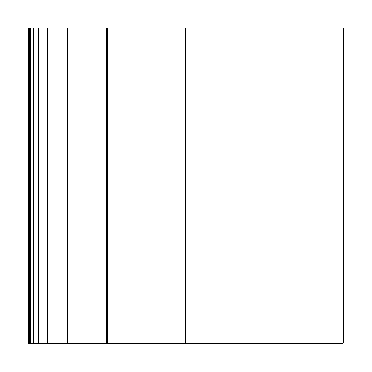
\begin{tikzpicture}
            \draw (0,0) -- (0,4);
            \draw (0,0) -- (4,0);
            \draw (4,4) -- (4,0);
            \draw (2,0) -- (2,4);
            \draw (1,0) -- (1,4);
            \draw (0.5,0) -- (0.5,4);
            \draw (0.25,0) -- (0.25,4);
            \draw (0.125,0) -- (0.125,4);
            \draw (0.0625,0) -- (0.0625,4);
            \draw (0.03125,0) -- (0.03125,4);
            \draw (0.015625,0) -- (0.015625,4);
        \end{tikzpicture}
        \caption{Conjunto $X$.}
        \label{fig:12_rel2}
    \end{figure}
    \noindent
    Si consideramos la aplicación $H:X\times [0,1]\to X$ dada por:
    \begin{equation*}
        H((x,y),t) = \left\{\begin{array}{ll}
                (x,(1-\nicefrac{t}{2})y)& \text{si\ } 0\leq t\leq \nicefrac{1}{2}\\
                (2(1-t)x,0)& \text{si\ } \nicefrac{1}{2}\leq t\leq 1
        \end{array}\right. 
    \end{equation*}
    Tenemos que:
    \begin{itemize}
        \item $H$ está bien definida, pues:
            \begin{equation*}
                \left(x,\left(1-\frac{\nicefrac{1}{2}}{2}\right)y\right) = (x,(1-1)y) = (x,0) = \left(2\left(1-\frac{1}{2}\right)x,0\right) 
            \end{equation*}
        \item $H$ es claramente continua en $X\times [0,\nicefrac{1}{2}]$ y en $X\times [\nicefrac{1}{2},1]$, por lo que por el Lema del Pegado obtenemos que $H$ es continua.
        \item $H$ cumple que:
            \begin{equation*}
                H((x,y),0) = (x,y),\quad H((x,y),1) = (0,0)\qquad \forall (x,y)\in X
            \end{equation*}
    \end{itemize}
    Por lo que hemos probado que $\{(0,0)\}$ es retracto de deformación de $X$, luego $X$ es contráctil.
\end{ejercicio}

\begin{ejercicio}
    Sea $f:\mathbb{R}\to \mathbb{R}^+$ una función continua. Definimos el conjunto:
    \begin{equation*}
        S_f = \left\{(x,y,z)\in \mathbb{R}^3: x^2+y^2 = {(f(z))}^{2}\right\}
    \end{equation*}
    \begin{enumerate}[label=\alph*)]
        \item Estudia el conjunto $S_f\cap \{z=z_0\}$ con $z_0\in \mathbb{R}$.

            Fijado $z_0\in \mathbb{R}$, tenemos que:
            \begin{equation*}
                S_f \cap \{z=z_0\} = \left\{(x,y,z)\in \mathbb{R}^3 : x^2+y^2 = {(f(z_0))}^{2}\right\}
            \end{equation*}
            que se trata de una circunferencia de centro $(0,0,z_0)$ y de radio $f(z_0)$. Podemos interpretar $S_f$ como el sólido de revolución obtenido a partir de la gráfica de $f$.
        \item Demuestra que cualesquiera dos conjuntos $S_f$ son homeomorfos entre sí.

            Sea $f:\mathbb{R}\to \mathbb{R}^+$ una función continua, consideramos $\Phi:S_f\to \bb{S}^1\times \mathbb{R}$ dada por:
            \begin{equation*}
                \Phi(x,y,z) = \left(\frac{x}{\sqrt{x^2+y^2}}, \frac{y}{\sqrt{x^2+y^2}}, z\right)
            \end{equation*}
            Así como la aplicación $\Psi:\bb{S}^1\times \mathbb{R}\to S_f$ dada por:
            \begin{equation*}
                \Psi(x,y,z) = (f(z)x, f(z)y, z)
            \end{equation*}
            Es claro que $\Phi$ y $\Psi$ son continuas, así como que:
            \begin{align*}
                &\Phi(\Psi(x,y,z)) = \Phi(f(z)x, f(z)y, z) = \\ 
                &=\left(\frac{f(z)x}{\sqrt{{(f(z)x)}^{2} + {(f(z)y)}^{2}}}, \frac{f(z)y}{\sqrt{{(f(z)x)}^{2} + {(f(z)y)}^{2}}}, z\right)\\
                &=\left(\frac{f(z)x}{\sqrt{{(f(z))}^{2}(x^2+y^2)}}, \frac{f(z)y}{\sqrt{{(f(z))}^{2}(x^2+y^2)}}, z\right) =\left(\frac{f(z)x}{\sqrt{{(f(z))}^{2}}}, \frac{f(z)y}{\sqrt{{(f(z))}^{2}}}, z\right)\\
                &=\left(\frac{f(z)x}{f(z)}, \frac{f(z)y}{f(z)}, z\right) = (x,y,z) \qquad \forall (x,y,z)\in \bb{S}^1\times \mathbb{R} \\
                &\Psi(\Phi(x,y,z)) = \Psi\left(\frac{x}{\sqrt{x^2+y^2}}, \frac{y}{\sqrt{x^2+y^2}}, z\right)= \left(\frac{f(z)x}{\sqrt{x^2+y^2}}, \frac{f(z)y}{\sqrt{x^2+y^2}}, z\right) \\
                &= \left(\frac{\sqrt{x^2+y^2}\cdot x}{\sqrt{x^2+y^2}}, \frac{\sqrt{x^2+y^2}\cdot y}{\sqrt{x^2+y^2}}, z\right)  = (x,y,z) \qquad \forall (x,y,z)\in S_f
            \end{align*}
            Por lo que $\Phi$ es un homeomorfismo.
        \item Calcula el grupo fundamental de $S_f$.

            Dado $(x,y,z)\in S_f$, el homeomorfismo $\Phi$ anterior induce un isomorfismo:
            \begin{equation*}
                \Phi_\ast:\pi_1(S_f,(x,y,z)) \to \pi_1(\bb{S}^1\times \mathbb{R},\Phi(x,y,z))
            \end{equation*}
            Y como $\pi_1(\bb{S}^1\times \mathbb{R},\Phi(x,y,z))\cong \mathbb{Z}$, tenemos que $\pi_1(S_f,(x,y,z))\cong \mathbb{Z}$.
    \end{enumerate}
\end{ejercicio}

\begin{ejercicio}
    Prueba que $\mathbb{R}\times \left[0,+\infty\right[$ no es homeomorfo a $\mathbb{R}^2$. ¿Son del mismo tipo de homotopía?\\

        \noindent
        Por reducción al absurdo, si $\mathbb{R}\times \left[0,+\infty\right[$ fuera homeomorfo a $\mathbb{R}^2$, existiría un homeomorfismo $f:\mathbb{R}\times \left[0,+\infty\right[\to \mathbb{R}^2$, por lo que la restricción de $f$ \newline$f\big|_{(\mathbb{R}\times \left[0,+\infty\right[)\setminus\{(0,0)\}}:(\mathbb{R}\times \left[0,+\infty\right[)\setminus\{(0,0)\}\to \mathbb{R}^2\setminus\{f(0,0)\}$ seguiría siendo un homeomorfismo, que induciría un isomorfismo entre sus grupos fundamentales.

                        Sin embargo, $(\mathbb{R}\times \left[0,+\infty\right[)\setminus\{(0,0)\}$ es un conjunto convexo, luego es simplemente conexo y $\mathbb{R}^2\setminus\{f(0,0)\}$ es homeomorfo a $\bb{S}^1$, que tiene $\mathbb{Z}$ como grupo fundamental, por lo que no pueden ser homeomorfos, contradicción que viene de suponer la que $\mathbb{R}\times \left[0,+\infty\right[$ y $\mathbb{R}^2$ son homeomorfos.\\

        \noindent
        Sí son del mismo tipo de homotopía. Para verlo, veamos que $\mathbb{R}\times \left[0,+\infty\right[$ es un retracto de deformación de $\mathbb{R}^2$, ya que definiendo $H:\mathbb{R}^2\times [0,1]\to \mathbb{R}^2$ dada por:
            \begin{equation*}
                H((x,y),t) = \left\{\begin{array}{ll}
                        (x,y) & \text{si\ } (x,y)\in \mathbb{R}\times \left[0,+\infty\right[ \\
                        (x, (1-t)y) & \text{si\ } (x,y)\in \mathbb{R}\times \left]-\infty, 0\right]
                \end{array}\right. 
            \end{equation*}
            Tenemos que:
            \begin{itemize}
                \item $H$ está bien definida, puesto que:
                    \begin{equation*}
                        (x,0) = (x,(1-t)0), \qquad \forall t\in [0,1]
                    \end{equation*}
                \item $H$ es continua, puesto que es continua en los cerrados $\mathbb{R}\times \left[0,+\infty\right[\times [0,1]$, $\mathbb{R}\times \left]-\infty,0\right]\times [0,1]$, luego podemos aplicar el Lema del Pegado.
                \item Se verifica que:
                    \begin{multline*}
                        H((x,y),0) = (x,y), \quad H((x,y),1) \in \mathbb{R}\times \left[0,+\infty\right[, \quad H((a,b),1) = (a,b) \\
                            \forall (x,y)\in \mathbb{R}^2, \quad \forall (a,b)\in \mathbb{R}\times \left[0,+\infty\right[
                    \end{multline*}
            \end{itemize}
            Por lo que $\mathbb{R}\times \left[0,+\infty\right[$ es retracto de deformación de $\mathbb{R}^2$ para $r:\mathbb{R}^2\to \mathbb{R}\times \left[0,+\infty\right[$ dada por $r(x,y) = H((x,y),1)$, que induce un isomorfismo entre grupos fundamentales $r_\ast:\pi_1(\mathbb{R}^2,(x,y))\to \pi_1(\mathbb{R}\times \left[0,+\infty\right[, r(x,y))\quad \forall (x,y)\in \mathbb{R}^2$, luego $\mathbb{R}\times \left[0,+\infty\right[$ y $\mathbb{R}^2$ son del mismo tipo de homotopía.
\end{ejercicio}

\begin{ejercicio}
    Sea $S$ un subespacio afín de $\mathbb{R}^n$ de dimensión $k\leq n-2$. Calcula $\pi_1(\mathbb{R}^n\setminus S)$.
\end{ejercicio}

\begin{ejercicio}
    Prueba que si $X$ es de Hausdorff y $A\subseteq X$ es un rectracto de $X$, entonces $A$ es cerrado en $X$. Deduce que una bola abierta en $\mathbb{R}^n$ no es un retracto de $\mathbb{R}^n$. ¿Lo es una bola cerrada?
\end{ejercicio}

\begin{ejercicio}
    En este ejercicio demostraremos que \textit{un abierto de $\mathbb{R}^2$ no puede ser homeomorfo a un abierto de $\mathbb{R}^n$ si} $n\geq 3$. Supongamos que $f:U\to V$ es un homeomorfismo entre abiertos no vacíos $U\subset \mathbb{R}^n$ y $V\subset \mathbb{R}^2$ con $n\geq 3$.
    \begin{enumerate}[label=\alph*)]
        \item Prueba que existen bolas abiertas $B_1\subset U$ y $B_2,B_2'\subset V$ (estas últimas con el mismo centro $y_0\in \mathbb{R}^2$) tales que $\overline{B_2'}\subset f(\overline{B_1})\subset \overline{B_2}$.
        \item Si $i:\overline{B_2'}\setminus \{y_0\}\to \overline{B_2}\setminus \{y_0\}$ es la inclusión, deduce de $a)$ que el homomorfismo inducido en cualquier punto $i_\ast$ es trivial.
        \item Prueba que $\overline{B_2'}\setminus \{y_0\}$ es un retracto de deformación de $\overline{B_2}\setminus \{y_0\}$. Concluye que $i_\ast$ es un isomorfismo no trivial, lo que contradice $b)$.
    \end{enumerate}
\end{ejercicio}

\begin{ejercicio}
    Demuestra que el sistema de ecuaciones:
    \begin{equation*}
        \left\{\begin{array}{l}
            x-\arctg(x^2-y^3) = 2 \\
            \cos(x) + \sen(xy^3) + e^x + e^{y^2} + \dfrac{1}{y} = -5
        \end{array}\right.
    \end{equation*}
    tiene al menos una solución en $\mathbb{R}^2$.
\end{ejercicio}

\begin{ejercicio}
    Sean $M$ una matriz cuadrada real de orden 3 por 3 cuyas entradas son números reales positivos
    y $f:\mathbb{R}^3\to \mathbb{R}^3$ la aplicación lineal $f(v)=Mv$. Demuéstrese que:
    \begin{enumerate}[label=\alph*)]
        \item El conjunto $A=\{(x,y,z)\in \bb{S}^2:x_1,x_2,x_3\geq 0\}$ es homeomorfo al disco cerrado $\overline{\bb{D}}$.
        \item La aplicación $g:A\to \bb{S}^2$ dada por $g(v) = \frac{f(v)}{|f(v)|}$ está bien definida y $g(A)\subset A$.
        \item $f$ tiene un valor propio real y positivo.
    \end{enumerate}
\end{ejercicio}

\begin{ejercicio}
    Teorema de Lusternik-Schnirelmann. Demuestra que si $\bb{S}^2$ es la unión de tres subconjuntos cerrados $C_1,C_2,C_3$, entonces alguno de ellos contiene dos puntos antípodas. Para ello prueba que la función $f:\bb{S}^2\to \bb{R}^2$ dada por
    \begin{equation*}
        f(x) = (dist(x,C_1), dist(x,C_2))
    \end{equation*}
    tiene un putno $x_0\in \bb{S}^2$ tal que $f(x_0) = f(-x_0)$, donde $dist(\cdot ,\cdot )$ denota la función distancia en $\mathbb{R}^3$.
\end{ejercicio}

\begin{ejercicio}
    Calcula $\pi_1(X)$ en los siguientes casos:
    \begin{enumerate}[label=\alph*)]
        \item $X=\bb{S}^2 \cup (\bb{D}\times \{0\})$.
        \item $X=(\bb{S}^1 \times [-1,1])\cup (\bb{D}\times \{-1,1\})$.
        \item $X = \{(x,y,z)\in \mathbb{R}^3 : x^2+y^2 = {(z+1)}^{2}, -1\leq z\leq 0\}\cup (\bb{S}^2 \cap \{z\geq 0\})$.
        \item $X = S_1 \cup S_2 \cup L$, donde $S_1,S_2$ son cerrados disjuntos simplemente conexos de $\mathbb{R}^n$ y $L\subset \mathbb{R}^n$ es un segmento tal que $L\cap S_i =\{x_i\}$, $i = 1,2$.
        \item $X\subset \mathbb{R}^3$ es la unión de una circunferencia y de una esfera que se tocan en un único punto.
        \item $X = \bb{S}^2\cup \{(x,y,z)\in \mathbb{R}^3 : y^2 + {(z-2)}^{2} = 1\}\cup \{(x,y,z)\in \mathbb{R}^3 : y^2 + {(z+2)}^{2}=1\}$.
        \item $X = S_1 \cup (\bb{S}^1 \times \{0\})\cup S_2$, donde $S_1$ y $S_2$ son, respectivamente, las esferas de radio 1 centradas en el $(0,-2,0)$ y en el $(0,2,0)$.
        \item $X\subset \mathbb{R}^2$ es la unión de las tres circunferencias de radio 1 centradas en los puntos $(-2,0)$, $(0,0)$ y $(2,0)$.
        \item $X = \bb{S}^1\cup [(-1,0), (1,0)]$.
    \end{enumerate}
\end{ejercicio}

\begin{ejercicio}
    Razona si son verdaderas o falsas las siguientes afirmaciones:
    \begin{enumerate}[label=\alph*)]
        \item Sean $\alpha_1,\alpha_2,\beta_1,\beta_2\in \Omega(X,x_0)$  con $[\alpha_1\ast \beta_1] = [\alpha_2\ast \beta_2]$. Entonces $[\alpha_1] = [\alpha_2]$ y $[\beta_1] = [\beta_2]$.\\

            Es falsa, puesto que si consideramos $X=\bb{S}^1$, $x_0 =(1,0)$, el arco:
            \begin{equation*}
                \alpha(t) = (\cos(2\pi t), \sen(2\pi t)) \qquad \forall t\in [0,1]
            \end{equation*}
            Y tomamos:
            \begin{equation*}
                \alpha_1 = \alpha = \beta_2, \qquad \alpha_2 = \varepsilon_{x_0} = \beta_1
            \end{equation*}
            Tenemos que $[\alpha_1] \neq [\alpha_2]$, $[\beta_1]\neq[\beta_2]$ y $[\alpha_1\ast \beta_1] = [\alpha_2\ast \beta_2]$.
        \item Sean $f:A\to Y$ una aplicación continua con $A\subset X$ y $X$ simplemente conexo. Si existe $F:X\to Y$ continua con $F\big|_A = f$, entonces $f_\ast$ es trivial.\\

            Es verdadera, como $F$ es una extensión de $f$, tenemos que $f\circ i = F$, es decir:
            \begin{figure}[H]
                \centering
                \shorthandoff{""}
                \begin{tikzcd}
                    {A} \arrow[r, "i", hook] \arrow[rr, "f", bend right=49] & {X} \arrow[r, "F"] & {Y}
                \end{tikzcd}
                \shorthandon{""}
            \end{figure}
            \noindent
            Y como cada una de ellas es continua, podemos inducir el diagrama a grupos fundamentales, obteniendo para cada $x_0\in A$:
            \begin{figure}[H]
                \centering
                \shorthandoff{""}
                \begin{tikzcd}
                    {\pi_1(A,x_0)} \arrow[r, "i_\ast", hook] \arrow[rr, "f_\ast", bend right] & {\pi_1(X,x_0)} \arrow[r, "F_\ast"] & {\pi_1(Y,f(x_0))}
                \end{tikzcd}
                \shorthandon{""}
            \end{figure}
            de donde:
            \begin{equation*}
                f_\ast([\alpha]_A) = F_\ast(i_\ast([\alpha]_{A})) = F_\ast({[\alpha]}_{X}) \AstIg F_\ast([\varepsilon_{x_0}]_{X}) = [\varepsilon_{f(x_0)}]_Y \qquad \forall [\alpha]_A \in \pi_1(A,x_0)
            \end{equation*}
            donde en $(\ast)$ hemos usado que $X$ es simplemente conexo.
        \item Si $f:X\to Y$ es continua y nulhomótopa, entonces $f_\ast$ es trivial.
        \item Si $f:X\to \bb{S}^n$ es continua y no sobreyectiva, entonces es nulhomótopa.
        \item Si $X$ es simplemente conexo y $A\subset X$ un rectracto de $X$, entonces $A$ es simplemente conexo.
        \item Si $f:X\to Y$ es continua e inyectiva con $f(x_0)=y_0$ entonces el homomorfismo $f_\ast:\pi_1(X,x_0)\to \pi_1(Y,y_0)$ es un monomorfismo.

            Falsa, puesto que la aplicación inclusión
            \Func{i}{\bb{S}^1}{\bb{R}^2}{x}{x}
            es continua e inyectiva, y si tomamos $x_0\in X$, $y_0 = f(x_0)$, tenemos el homomorfismo $i_\ast:\pi_1(\bb{S}^1,x_0)\to \pi_1(\mathbb{R}^2, x_0)$ que no es inyectivo, puesto que:
            \begin{equation*}
                \pi_1(\bb{S}^1,x_0) \cong \mathbb{Z}, \qquad \pi_1(\mathbb{R}^2,x_0)\cong \{1\}
            \end{equation*}
        \item Sea $f:X\to Y$ una equivalencia homotópica y $A\subset X$. La restricción $f\big|_A:A\to f(A)$ es una equivalencia homotópica.
        \item $\bb{S}^1$ no tiene ningún retracto de deformación $A\neq \bb{S}^1$.
        \item Existe un homeomorfismo de $\mathbb{R}^2$ que intercambia las componentes conexas de $\mathbb{R}^2\setminus \bb{S}^1$.
        \item Si $A$ es un retracto del disco unidad cerrado de $\mathbb{R}^2$, entonces toda aplicación continua $f:A\to A$ tiene al menos un punto fijo.
    \end{enumerate}
\end{ejercicio}
